\documentclass[handout,xcolor=pdftex,dvipsnames,table]{beamer}\usepackage[]{graphicx}\usepackage[]{color}
%% maxwidth is the original width if it is less than linewidth
%% otherwise use linewidth (to make sure the graphics do not exceed the margin)
\makeatletter
\def\maxwidth{ %
  \ifdim\Gin@nat@width>\linewidth
    \linewidth
  \else
    \Gin@nat@width
  \fi
}
\makeatother

\definecolor{fgcolor}{rgb}{0.345, 0.345, 0.345}
\newcommand{\hlnum}[1]{\textcolor[rgb]{0.686,0.059,0.569}{#1}}%
\newcommand{\hlstr}[1]{\textcolor[rgb]{0.192,0.494,0.8}{#1}}%
\newcommand{\hlcom}[1]{\textcolor[rgb]{0.678,0.584,0.686}{\textit{#1}}}%
\newcommand{\hlopt}[1]{\textcolor[rgb]{0,0,0}{#1}}%
\newcommand{\hlstd}[1]{\textcolor[rgb]{0.345,0.345,0.345}{#1}}%
\newcommand{\hlkwa}[1]{\textcolor[rgb]{0.161,0.373,0.58}{\textbf{#1}}}%
\newcommand{\hlkwb}[1]{\textcolor[rgb]{0.69,0.353,0.396}{#1}}%
\newcommand{\hlkwc}[1]{\textcolor[rgb]{0.333,0.667,0.333}{#1}}%
\newcommand{\hlkwd}[1]{\textcolor[rgb]{0.737,0.353,0.396}{\textbf{#1}}}%

\usepackage{framed}
\makeatletter
\newenvironment{kframe}{%
 \def\at@end@of@kframe{}%
 \ifinner\ifhmode%
  \def\at@end@of@kframe{\end{minipage}}%
  \begin{minipage}{\columnwidth}%
 \fi\fi%
 \def\FrameCommand##1{\hskip\@totalleftmargin \hskip-\fboxsep
 \colorbox{shadecolor}{##1}\hskip-\fboxsep
     % There is no \\@totalrightmargin, so:
     \hskip-\linewidth \hskip-\@totalleftmargin \hskip\columnwidth}%
 \MakeFramed {\advance\hsize-\width
   \@totalleftmargin\z@ \linewidth\hsize
   \@setminipage}}%
 {\par\unskip\endMakeFramed%
 \at@end@of@kframe}
\makeatother

\definecolor{shadecolor}{rgb}{.97, .97, .97}
\definecolor{messagecolor}{rgb}{0, 0, 0}
\definecolor{warningcolor}{rgb}{1, 0, 1}
\definecolor{errorcolor}{rgb}{1, 0, 0}
\newenvironment{knitrout}{}{} % an empty environment to be redefined in TeX

\usepackage{alltt} 

\usecolortheme[RGB={0,0,144}]{structure}
%\usetheme{AnnArbor}\usecolortheme{beaver}
\usetheme{CambridgeUS}\usecolortheme{dolphin}

\usepackage{graphicx}
\usepackage[space]{grffile}
\usepackage{verbatim,xmpmulti,color,multicol,multirow}
\setlength{\unitlength}{\textwidth}  % measure in textwidths
\usepackage[normalem]{ulem}
\usepackage{amssymb,amsmath,latexsym}
\usepackage{booktabs}
\usepackage{array}
\newcolumntype{L}{>{$}l<{$}}
\newcolumntype{C}{>{$}c<{$}}
\newcolumntype{R}{>{$}r<{$}}
\newcommand{\nm}[1]{\textnormal{#1}}


%\usepackage{beamerthemesplit}
\setbeamertemplate{navigation symbols}{}
\setbeamertemplate{caption}[numbered]
%\setbeamercolor{alerted text}{fg=red}
%\setbeamertemplate{block body theorem}{bg=orange}
\setkeys{Gin}{width=0.6\textwidth}


%\SweaveOpts{concordance=TRUE}







\title[RNASeq Analysis]{Analyze RNASeq Data from G9P2 RFI (Residual Feed Intake) Lines Using QuasiSeq Package (paired end read)}


% \author[Yet Nguyen, Dan Nettleton]{Yet Nguyen \and Dan Nettleton}
% \institute[ISU]{Iowa State University}

%
\IfFileExists{upquote.sty}{\usepackage{upquote}}{}

\begin{document}
\frame{\maketitle}
\frame {
\frametitle{Table of Contents}
\begin{itemize}
\setlength{\itemsep}{.2in}
\item[1.] Data Summary
\item[2.] Model Selection Stragegies
\begin{itemize}
\item Number of genes with pvalues less than 0.05
\item Distance between Grenander CDF Estimator to Uniform CDF using
\begin{itemize}
\item Anderson-Darling Statistics
\item Cram{\'e}r-Von-Mises statistics
\item Kolmogorov-Smirnov statistics 
\end{itemize}
\end{itemize}
\item[3.] Results
\end{itemize}
}


\section{Data Summary}
\begin{frame}[fragile]
\frametitle{RNASeq Data Summary}
\begin{itemize}
\setlength{\itemsep}{.25in}
\item RNASeq data set is a  25320 $\times$ 31 table of count data  corresponding to 25320 genes of 31  pigs from 2 Lines: high RFI Line and low RFI Line, and 2 Diets: high energy diet (Diet 1) and low energy diet (Diet 2).

\item  For Diet 1, the RNA data are from 7 low RFI line pigs and 8  high RFI line pigs. 
For Diet 2, the RNA data are from 8 low RFI line pigs and 8  high RFI line pigs.
 
\end{itemize}
 

\end{frame}




%%%%%%%%%%%%%%%%
\frame{
\frametitle{Metadata Summary}
\begin{itemize}
\setlength{\itemsep}{.25in}
\item The available metadata consists of infomation of  9 covariates for 31 samples of 31 pigs.

\begin{itemize}
\item Factors: Diet (2 levels), Line (2 levels), Block (4 levels), Blockorder (8 levels).
\item Quantitative covariates: RFI (RFI values) , RINb (RNA Integrity Number before globin depletion), RINa (RNA Integrity Number after globin depletion), Concb (RNA Concentration before globin depletion), Conca(RNA Concentration after globin depletion).
\end{itemize}
\item CBC (Complete Blood Count) data:  neutrophils, lymphocytes, monocytes, eosinophils, and basophils. The CBC covariates are in model in the form of log2 transformation.
\end{itemize}
}
%%%%%%%%%%%%%%%%%%%%%%%%%%%%%%%%%%%%%%%%%%%5

\frame{
\frametitle{Number of Genes Used in Analysis}
\begin{itemize}

\setlength{\itemsep}{.25in}


\item Models with metadata covariates and with CBC covariates: The number of genes analyzed is 12280. Those are genes with average counts greater than 8 and for which there are at least four samples with non-zero counts. 
\end{itemize}
}


%%%%%%%%%%%%%%%%%%%%%%%%%%%%%%%%%%%%%%%%%%%%%%%%%%%%%
\section{Model Selection}
\begin{frame}
\frametitle{Model Selection Criteria}
Starting model includes all  covariates of interest. For each covariate, 
\begin{itemize}
\setlength{\itemsep}{.2in}
\item We conduct a Likelihood Ratio Test using QuasiSeq of the full model vs. the reduced model obtained from the full model by deleting the considered covariate. We collect the set of pvalues of all genes from the tests. 

\item Obtain the number of genes with pvalues less than or equal 0.05. 
\item Obtain Grenander CDF estimator of the empirical CDF of those pvalues.
\item Obtain the Anderson-Darling statistics, Cram{\'e}r-Von-Mises statistics, and Kolmogorov-Smirnov statistics between the Grenander CDF and uniform CDF.
\end{itemize}
Exclude the covariate corresponding to the smallest value for most of the above criteria.
\end{frame}
\begin{frame}[fragile]
\frametitle{Backward Model Selection}
\begin{figure}[h!]
    \centering
    %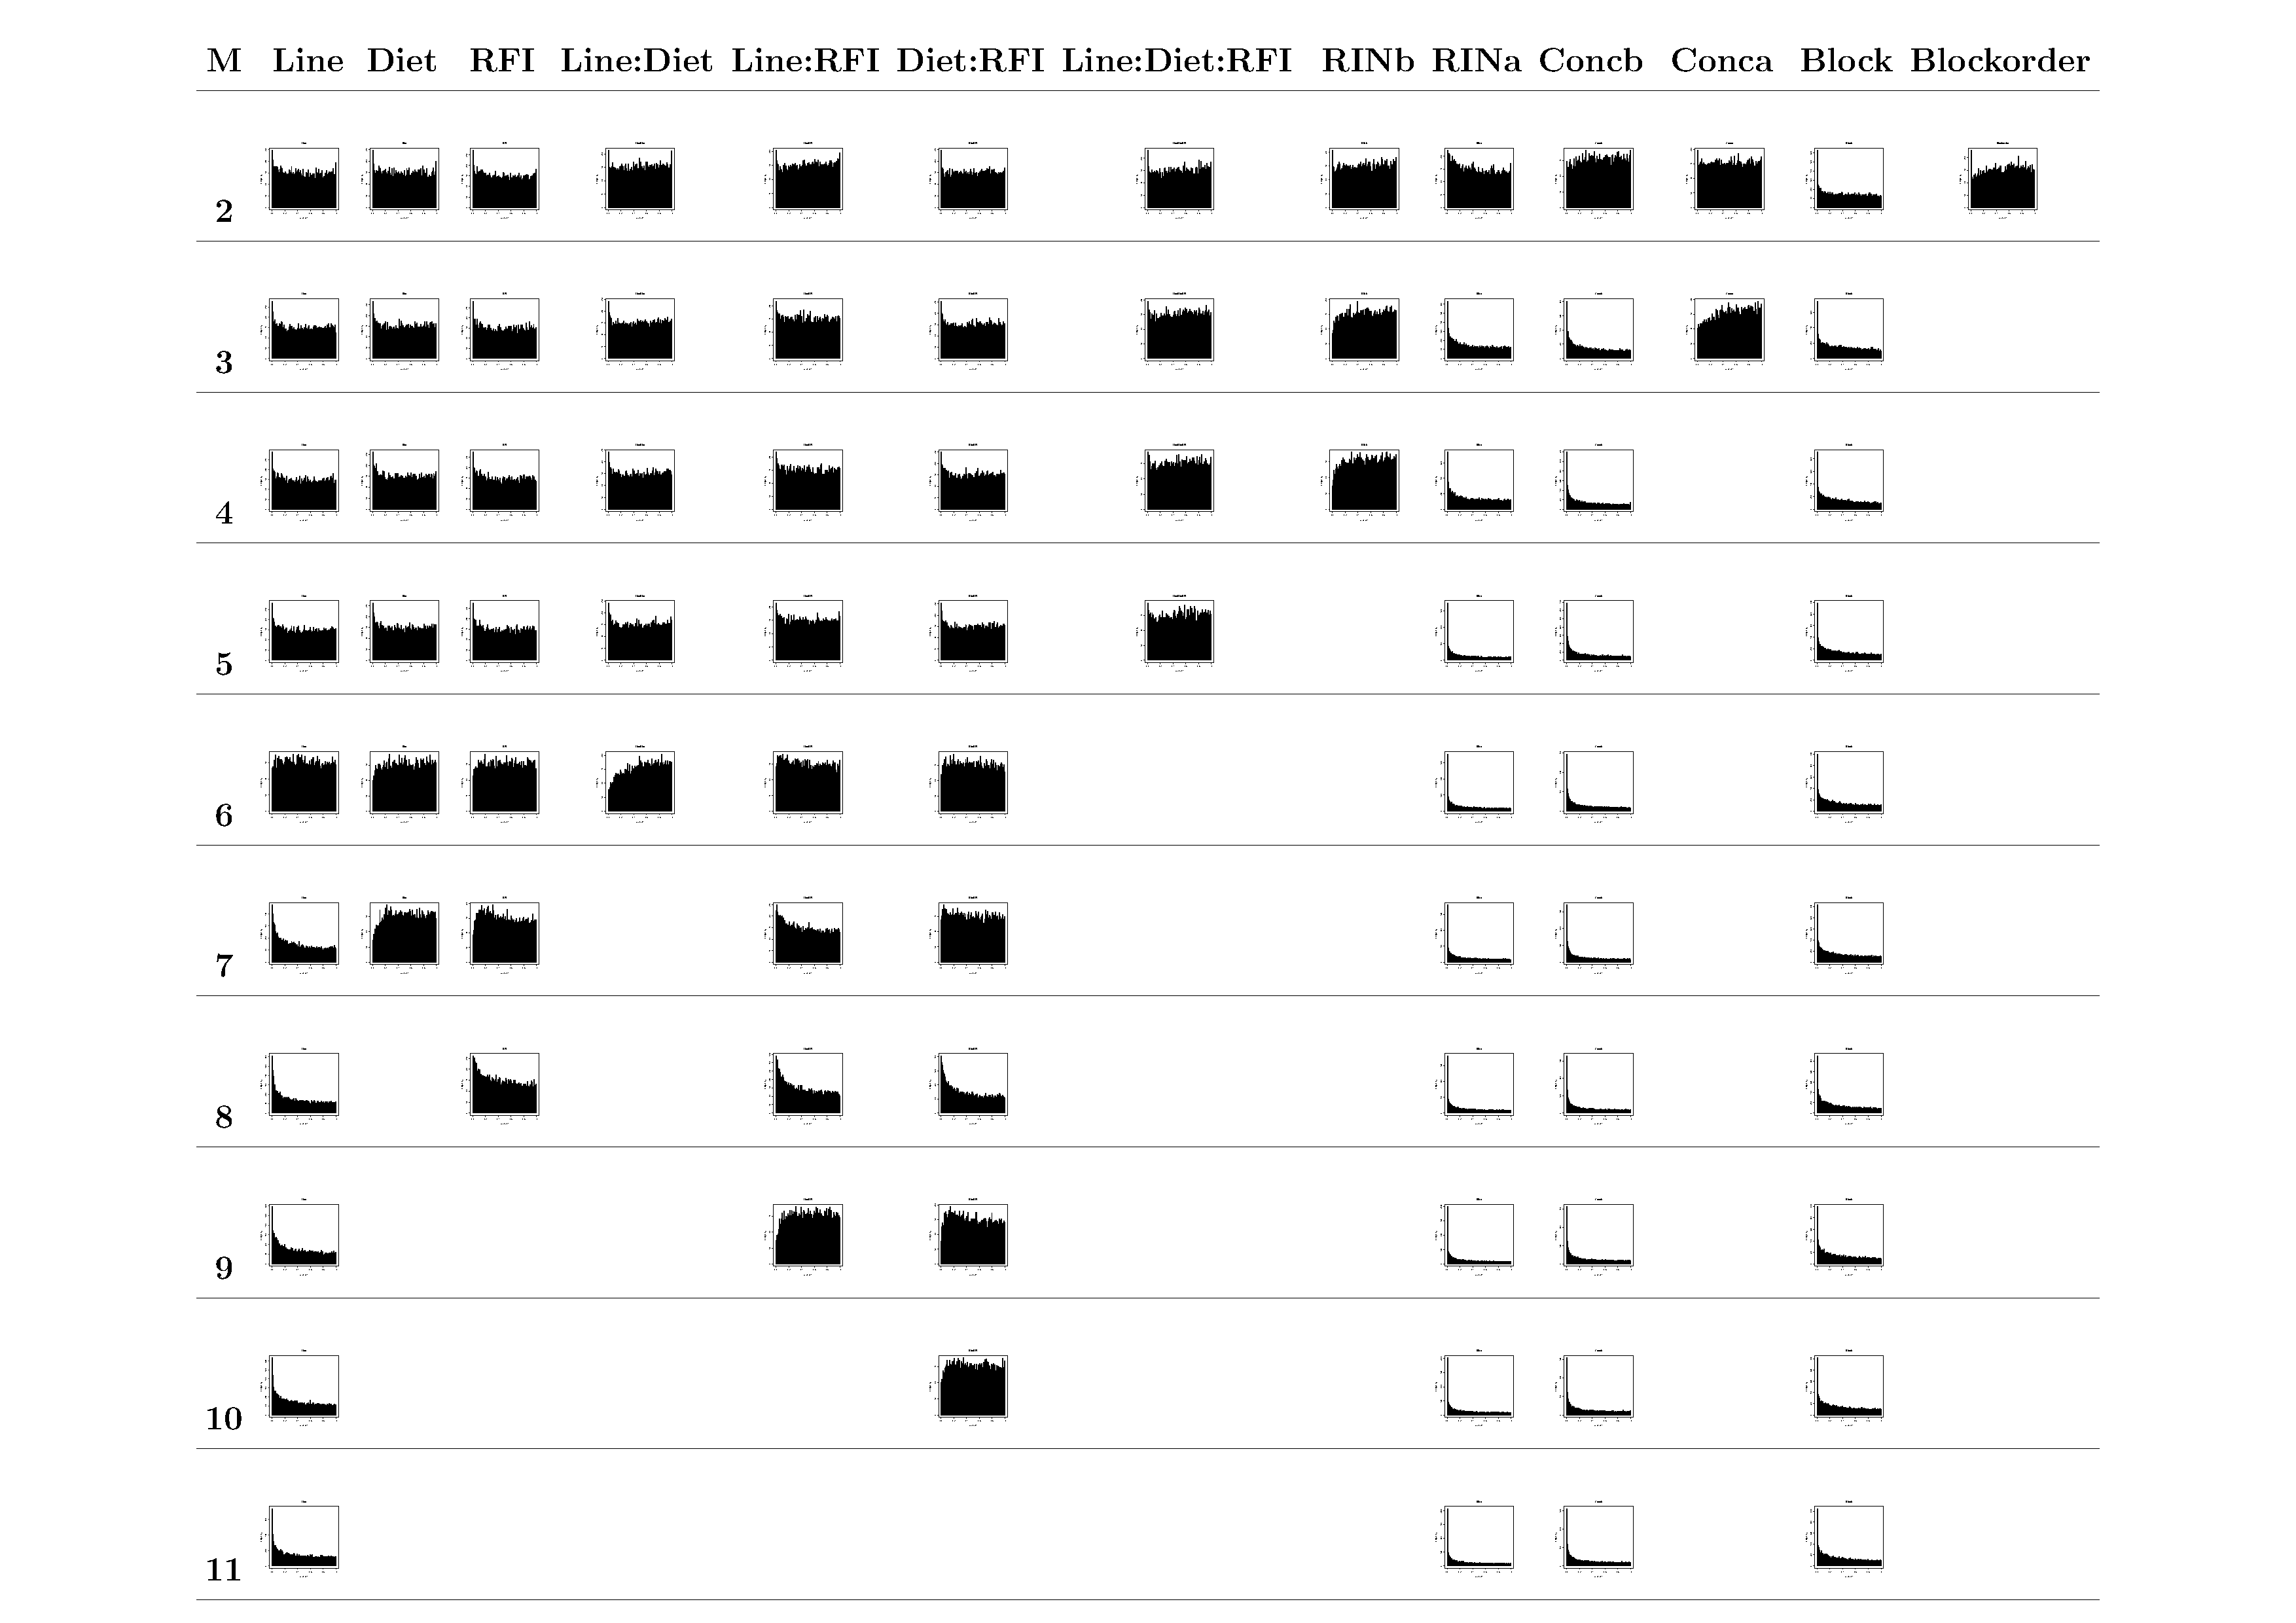
\includegraphics[width=\textwidth,height=0.8\textheight,keepaspectratio]{/home/ntyet/research/RFI-newdata/analysis/rfi/Plot06_26_2014_1.pdf}
    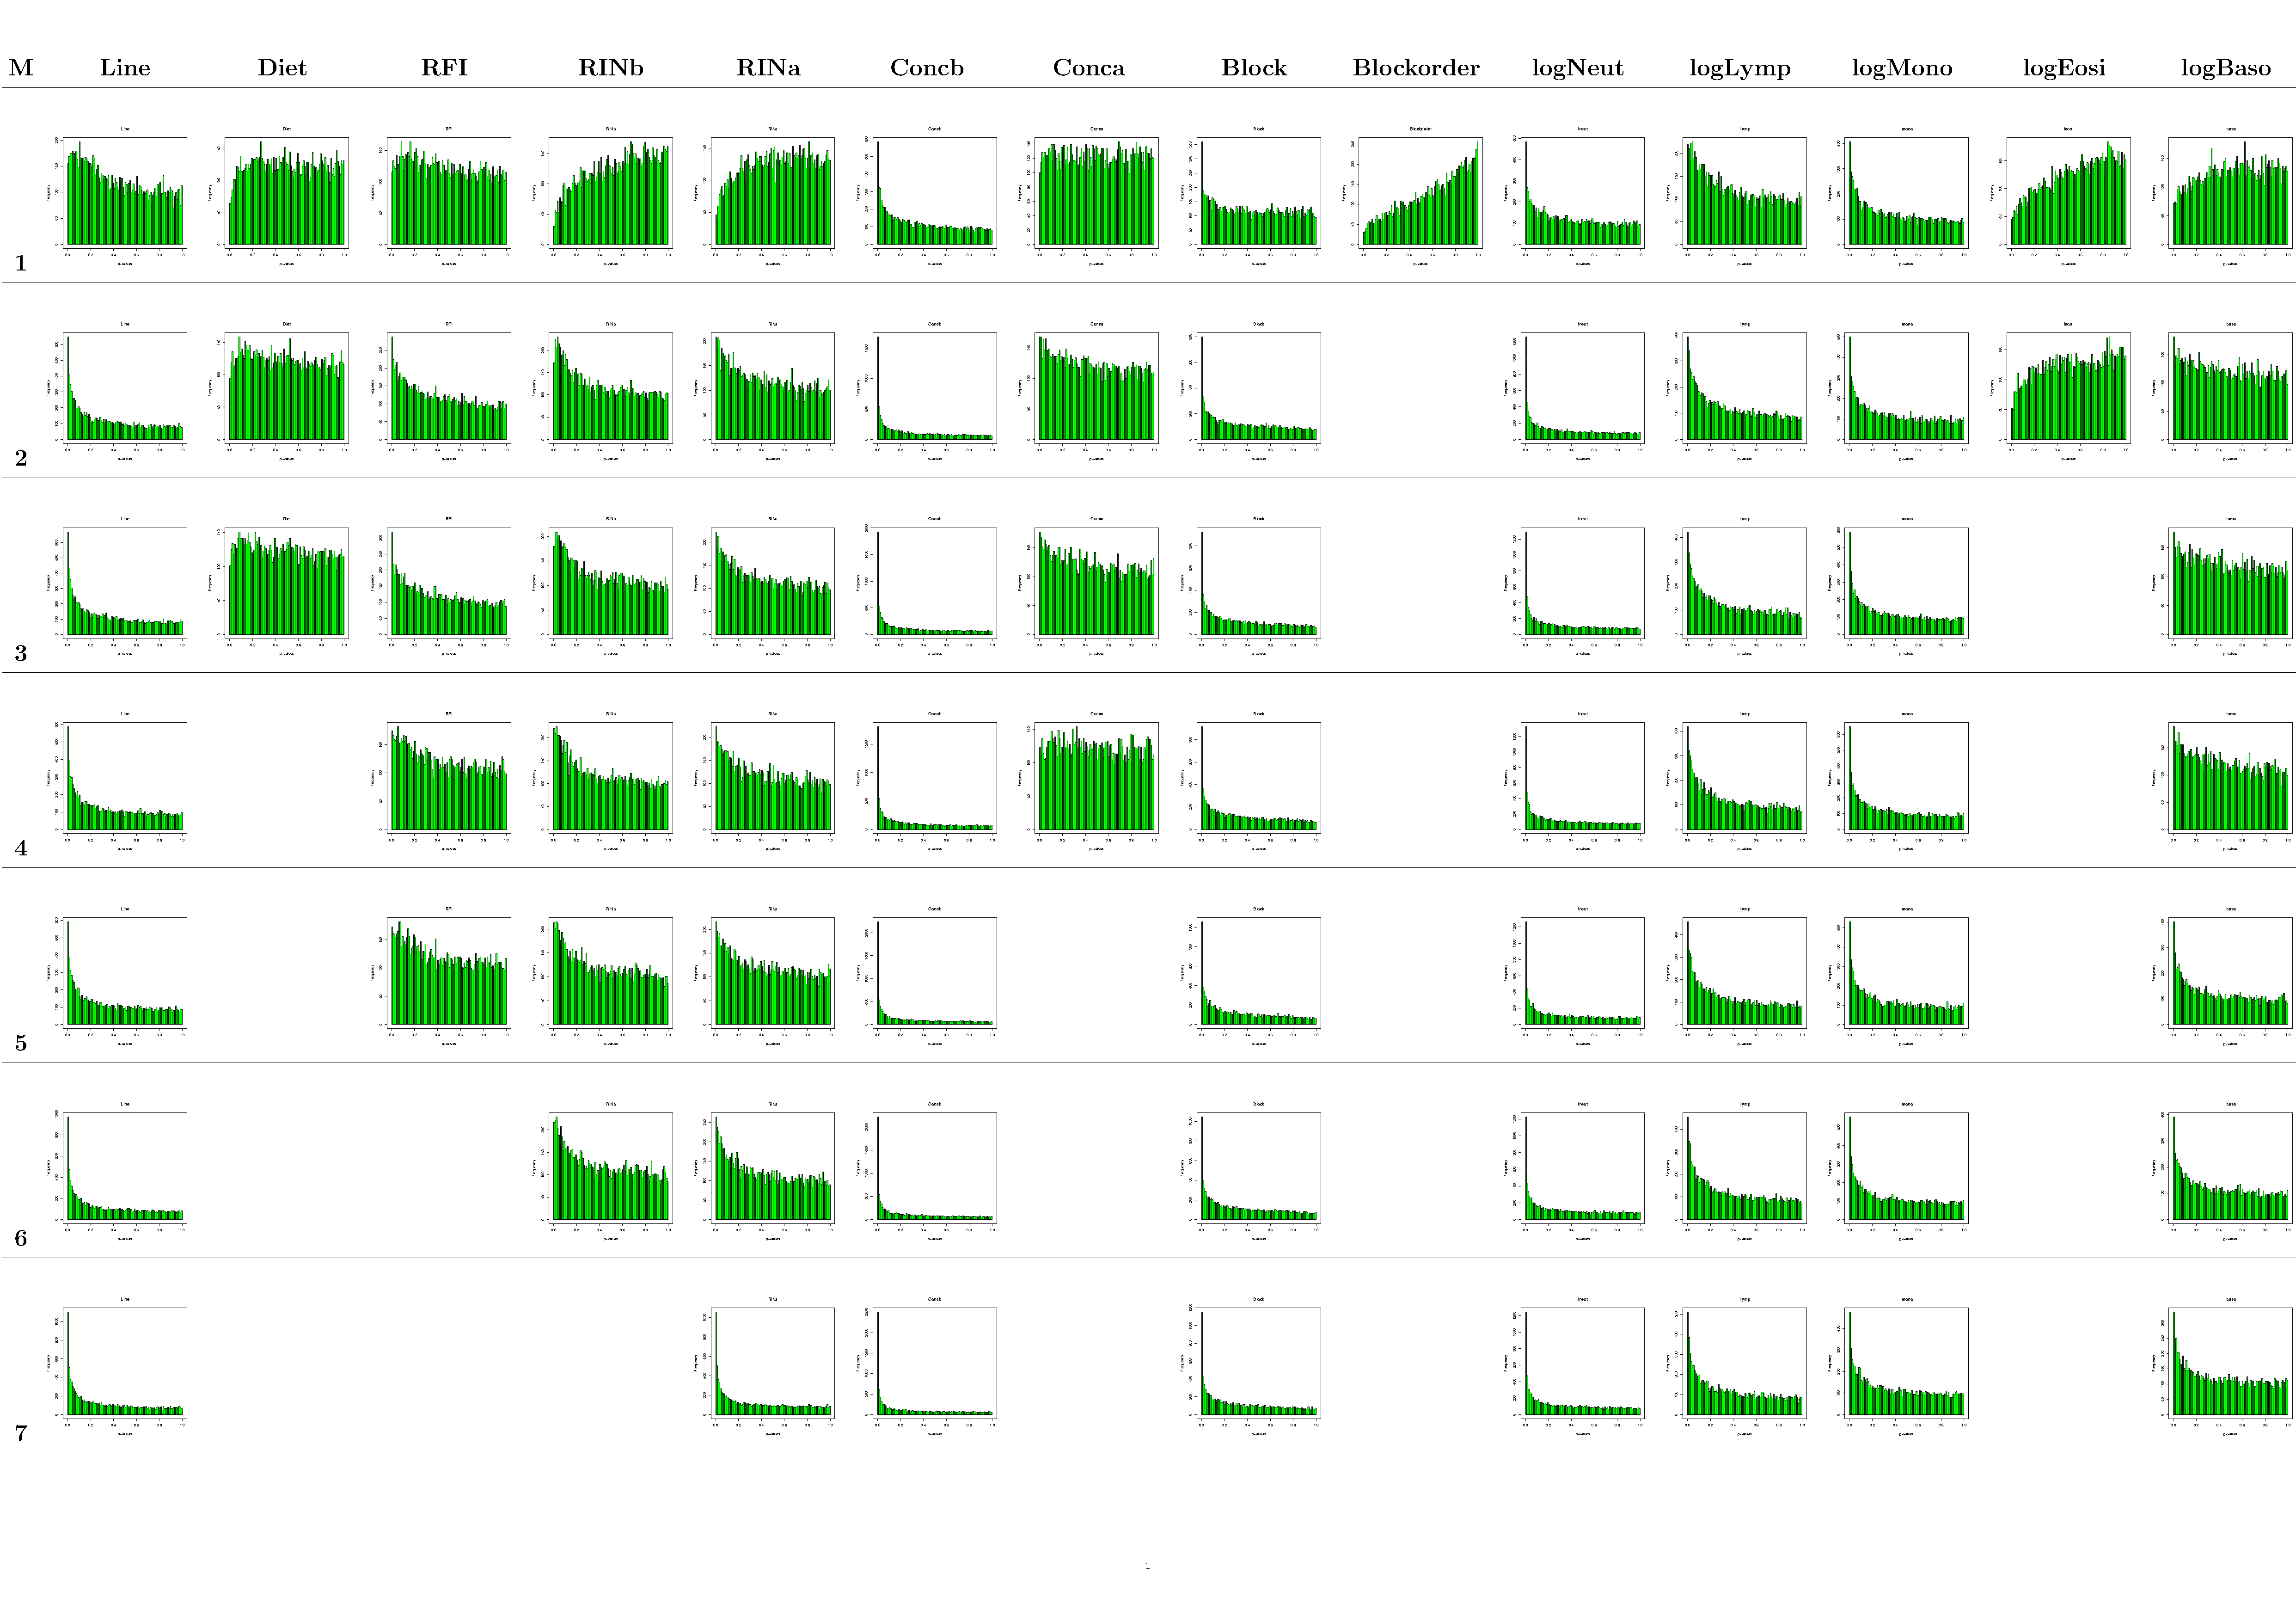
\includegraphics[width=\textwidth,height=1.4\textheight,keepaspectratio]{Plot07_022014_rficbcdat2.pdf}
    \end{figure}
\end{frame}
\section{Results}
\begin{frame}[fragile]
\frametitle{Results of Model 7}
\begin{itemize}
\item 
Estimated number of DE Genes between two RFI Lines
\begin{knitrout}\footnotesize
\definecolor{shadecolor}{rgb}{0.969, 0.969, 0.969}\color{fgcolor}\begin{kframe}
\begin{verbatim}
## [1] 4990
\end{verbatim}
\end{kframe}
\end{knitrout}


\item When FDR is controlled at 0.05, 0.10, 0.15, the number of DE Genes between two RFI Lines (DEGs) and the number of DE Genes between two RFI Lines with log2(fold change) at least 1 (log2(FC) $\geq 1$) are shown in the table below
% latex table generated in R 3.1.0 by xtable 1.7-3 package
% Tue Jul 15 16:43:39 2014
\begin{table}[ht]
\centering
\begin{tabular}{rrr}
  \hline
FDR & DEGs & $\mbox{log2(FC)}\geq 1$ \\ 
  \hline
0.05 & 771 &  61 \\ 
  0.10 & 1837 &  92 \\ 
  0.15 & 2936 & 101 \\ 
   \hline
\end{tabular}
\end{table}


\end{itemize}
\end{frame}

\end{document}
